\documentclass[czech]{beamer}
\usepackage{helvet}
\renewcommand{\familydefault}{\sfdefault}
\usepackage[T1]{fontenc}
\usepackage[utf8]{inputenc}
\usepackage[active]{srcltx}
\usepackage{babel}
\usepackage{array}
\usepackage{amstext}
\usepackage{amssymb}
\usepackage{graphicx}
\ifx\hypersetup\undefined
  \AtBeginDocument{%
    \hypersetup{pdfusetitle,
 bookmarks=true,bookmarksnumbered=false,bookmarksopen=false,
 breaklinks=false,pdfborder={0 0 1},backref=false,colorlinks=false}
  }
\else
  \hypersetup{pdfusetitle,
 bookmarks=true,bookmarksnumbered=false,bookmarksopen=false,
 breaklinks=false,pdfborder={0 0 1},backref=false,colorlinks=false}
\fi

\makeatletter

% Specific LaTeX commands.
%% Because html converters don't know tabularnewline
\providecommand{\tabularnewline}{\\}

%%%%%%%%%%%%%%%%%%%%%%%%%%%%%% Textclass specific LaTeX commands.
% this default might be overridden by plain title style
\newcommand\makebeamertitle{\frame{\maketitle}}%
% (ERT) argument for the TOC
\AtBeginDocument{%
  \let\origtableofcontents=\tableofcontents
  \def\tableofcontents{\@ifnextchar[{\origtableofcontents}{\gobbletableofcontents}}
  \def\gobbletableofcontents#1{\origtableofcontents}
}
\newenvironment{lyxcode}
  {\par\begin{list}{}{
    \setlength{\rightmargin}{\leftmargin}
    \setlength{\listparindent}{0pt}% needed for AMS classes
    \raggedright
    \setlength{\itemsep}{0pt}
    \setlength{\parsep}{0pt}
    \normalfont\ttfamily}%
   \def\{{\char`\{}
   \def\}{\char`\}}
   \def\textasciitilde{\char`\~}
   \item[]}
  {\end{list}}

%%%%%%%%%%%%%%%%%%%%%%%%%%%%%% User specified LaTeX commands.
\date{}
\beamertemplateshadingbackground{red!5}{structure!5}

\usepackage{beamerthemecambridgeus}
\usepackage{pgfnodes,pgfarrows,pgfheaps}
\usepackage {multicol}

\beamertemplatetransparentcovereddynamicmedium
% Added by lyx2lyx
\setlength{\parskip}{\smallskipamount}
\setlength{\parindent}{0pt}

\makeatother

\begin{document}
\title{Datové struktury. }
\subtitle{Datové typy. Základní a odvozené datové struktury.}
\author{Tomáš Bayer | bayertom@fsv.cvut.cz}
\institute{Katedra geomatiky, fakulta stavební ČVUT.}
\makebeamertitle
\begin{frame}{Obsah přednášky}

\tableofcontents{}

\end{frame}

\section{Datové typy}
\begin{frame}[plain]{1. Základní datové typy}

{\scriptsize Logické, celočíselné, reálné a znakové.}{\scriptsize\par}

{\scriptsize Existují prakticky ve všech programovacích jazycích.}{\scriptsize\par}

{\scriptsize Definován rozsah hodnot v bajtech (velikost uloženého
čísla).}{\scriptsize\par}

{\scriptsize\medskip{}
}{\scriptsize\par}

{\scriptsize Python dynamicky typovaný jazyk, datový typ u proměnné
nemusíme uvádět.}{\scriptsize\par}

{\scriptsize Avšak uvnitř silná typová kontrola.}{\scriptsize\par}

{\scriptsize\medskip{}
}{\scriptsize\par}

{\scriptsize\textbf{Celočíselné datové typy: }}{\scriptsize\par}

{\scriptsize Reprezentace diskrétních jevů, výpočty ``bezchybné'':
}{\scriptsize\texttt{int}}{\scriptsize , }{\scriptsize\texttt{long}}{\scriptsize .}{\scriptsize\par}

{\scriptsize Velikost shora neomezená (není běžné u jiných programovacích
jazyků).}{\scriptsize\par}

{\scriptsize\medskip{}
}{\scriptsize\par}

{\scriptsize\textbf{Logické datové typy:}}{\scriptsize{} }{\scriptsize\par}

{\scriptsize Reprezentace stavů pravda/nepravda: }{\scriptsize\texttt{Boolean}}{\scriptsize\medskip{}
}{\scriptsize\par}

{\scriptsize\textbf{Reálné datové typy:}}{\scriptsize{} }{\scriptsize\par}

{\scriptsize Reprezentace spojitých jevů: }{\scriptsize\texttt{float}}{\scriptsize ,
}{\scriptsize\texttt{double}}{\scriptsize .}{\scriptsize\par}

{\scriptsize Velikost shora/zdola omezená, výpočty zatíženy chybou.}{\scriptsize\par}

{\scriptsize Standardizace IEEE 754.}{\scriptsize\par}

{\scriptsize\medskip{}
}{\scriptsize\par}

{\scriptsize\textbf{Znakové typy:}}{\scriptsize\par}

{\scriptsize Vyjádření textových informací, znak: }{\scriptsize\texttt{char}}{\scriptsize ,
slovo: }{\scriptsize\texttt{string}}{\scriptsize .}{\scriptsize\par}

{\scriptsize Znak lze reprezentovat celým číslem.}{\scriptsize\par}

{\scriptsize ASCII nebo UNICODE sady.}{\scriptsize\par}
\end{frame}

\begin{frame}[plain]{2. Práce s literály}

{\scriptsize\emph{Literál: }}{\scriptsize přímý zápis hodnoty učitého
typu v programovacím jazyce.\medskip{}
}{\scriptsize\par}

{\scriptsize\emph{Celé číslo}}{\scriptsize{} :}{\scriptsize\par}
\begin{lyxcode}
{\scriptsize 123456789}{\scriptsize\par}
\end{lyxcode}
{\scriptsize\emph{Reálné číslo: }}{\scriptsize pevná/plovoucí řádová
čárka, stejná absolutní/relativní přesnost}{\scriptsize\par}
\begin{lyxcode}
{\scriptsize 3.14159~~~~~~~1.0e-15~~~~~~~~~\#FX~vs~FP}{\scriptsize\par}
\end{lyxcode}
{\scriptsize Malá čísla méně přesná, problematické při některých aritmetických
operacích.\medskip{}
}{\scriptsize\par}

{\scriptsize\emph{Nečíselný výsledek, NaN (Not a Number):}}{\scriptsize\par}

{\scriptsize Výsledek operace není definován (např. odmocnina ze záporného
čísla).}{\scriptsize\par}
\begin{lyxcode}
{\scriptsize math.sqrt(-1)~}{\scriptsize\par}

{\scriptsize >\textcompwordmark >\textcompwordmark >~ValueError:~math~domain~error}{\scriptsize\par}
\end{lyxcode}
{\scriptsize\emph{Nekonečno, Inf (Infinity):}}{\scriptsize\par}

{\scriptsize Výsledek aritmetických operací (např. dělení 0).}{\scriptsize\par}
\begin{lyxcode}
{\scriptsize math.sqrt(1/0)~}{\scriptsize\par}

{\scriptsize >\textcompwordmark >\textcompwordmark >~ZeroDivisionError:~division~by~zero}{\scriptsize\par}
\end{lyxcode}
{\scriptsize\emph{Logická hodnota:}}{\scriptsize\par}
\begin{lyxcode}
{\scriptsize True~~~~~~~False}{\scriptsize\par}
\end{lyxcode}
{\scriptsize\emph{Řetězce}}{\scriptsize : single, double, tripple quoted}{\scriptsize\par}
\begin{lyxcode}
{\scriptsize 'Hello'~~~~~~\textquotedbl Hello\textquotedbl ~~}{\scriptsize\par}

{\scriptsize\textquotedbl\textquotedbl\textquotedbl We~are~ready~to~~~~~~\#Viceradkovy~text}{\scriptsize\par}

{\scriptsize ~~~~~learn~\textquotedbl Python\textquotedbl\textquotedbl\textquotedbl )}{\scriptsize\par}
\end{lyxcode}
\end{frame}

\begin{frame}[plain]{3. IEEE 754 (1985)}

{\tiny Definice standardů pro aritmetiku s reálnými čísly (plovoucí
řádová čárka).}{\tiny\par}

{\tiny Implementováno v programovacích jazycích.}{\tiny\par}

{\tiny\medskip{}
}{\tiny\par}

{\tiny Nejdůležitější body:}{\tiny\par}
\begin{itemize}
\item {\tiny\emph{Přesnost}}{\tiny\par}

{\tiny Jednoduchá přesnost (32 bit), dvojitá (64 bit), dvojitá rozšířená
(80 bit).}{\tiny\par}
\begin{center}
{\tiny{}%
\begin{tabular}{|c|c|c|c|}
\hline 
{\tiny Typ} & {\tiny Platné cifry} & {\tiny Reprezentace} & {\tiny Chyba}\tabularnewline
\hline 
\hline 
{\tiny\texttt{float}} & {\tiny 7} & {\tiny 32 bit} & {\tiny$2.38\cdot10^{-7}$}\tabularnewline
\hline 
{\tiny\texttt{double}} & {\tiny 15} & {\tiny 64 bit} & {\tiny$1.42\cdot10^{-14}$}\tabularnewline
\hline 
\end{tabular}}{\tiny\par}
\par\end{center}
\item {\tiny\emph{Nečíselný výsledek, NaN (Not a Number).}}{\tiny\par}

{\tiny Výsledek operace není definován (např. odmocnina ze záporného
čísla).}{\tiny\par}

\end{itemize}
\begin{lyxcode}
{\tiny math.sqrt(-1)~}{\tiny\par}

{\tiny >\textcompwordmark >\textcompwordmark >~ValueError:~math~domain~error}{\tiny\par}
\end{lyxcode}
\begin{itemize}
\item {\tiny\emph{Nekonečno, Inf (Infinity)}}{\tiny\par}

{\tiny Výsledek aritmetických operací (např. dělení 0).}{\tiny\par}

\end{itemize}
\begin{lyxcode}
{\tiny math.sqrt(1/0)~}{\tiny\par}

{\tiny >\textcompwordmark >\textcompwordmark >~ZeroDivisionError:~division~by~zero}{\tiny\par}
\end{lyxcode}
\begin{itemize}
\item {\tiny\emph{Přetečení, podtečení}}{\tiny\par}

{\tiny Mezní hodnoty: $x_{min}=2^{-126}$, $x_{max}=2^{127}$.\medskip{}
}{\tiny\par}

{\tiny$x<0\wedge x<-x_{max}$: Negative Overflow,}{\tiny\par}

{\tiny$x<0\wedge x>-x_{min}$: Negative Underflow,}{\tiny\par}

{\tiny$x>0\wedge x<x_{min}$: Positive Underflow,}{\tiny\par}

{\tiny$x>0\wedge x>x_{max}$: Positive Overflow.}{\tiny\par}
\end{itemize}
\end{frame}

\begin{frame}[plain]{4. Problémy při práci s reálnými čísly}

{\tiny\textbf{\textcolor{brown}{Problém 1: Zaokrouhlení při matematikých
operacích}}}{\tiny\par}

{\tiny V podmínkách místo a==b používat abs(a-b)<eps}{\tiny\par}
\begin{lyxcode}
{\tiny acos(cos(1))==1}{\tiny\par}

{\tiny >\textcompwordmark >\textcompwordmark >~False}{\tiny\par}
\end{lyxcode}
{\tiny\textbf{\textcolor{brown}{Problém 2: Odečtení malého čísla od
čísla}}}{\tiny\par}

{\tiny Výsledek operace je špatný.}{\tiny\par}
\begin{lyxcode}
{\tiny x~=~1.0}{\tiny\par}

{\tiny y~=~0.0000000000000000005}{\tiny\par}

{\tiny z~=~x~-~y}{\tiny\par}

{\tiny >\textcompwordmark >\textcompwordmark >~1.0}{\tiny\par}
\end{lyxcode}
{\tiny\textbf{\textcolor{brown}{Problém 3: Přičtení malého čísla k
velkému číslu}}}{\tiny\par}

{\tiny Porovnání dá špatný výsledek.}{\tiny\par}
\begin{lyxcode}
{\tiny x~=~1.0e20}{\tiny\par}

{\tiny x~==~x~+~1}{\tiny\par}

{\tiny >\textcompwordmark >\textcompwordmark >~True}{\tiny\par}
\end{lyxcode}
{\tiny\textbf{\textcolor{brown}{Problém 4: Asociativita pro malá a
velká čísla}}}{\tiny\par}

{\tiny Zdánlivá nefunkčnost asociativity.}{\tiny\par}
\begin{lyxcode}
{\tiny a~=~1}{\tiny\par}

{\tiny b~=~1e20}{\tiny\par}

{\tiny c~=~-1e20}{\tiny\par}

{\tiny a~+~(~b~+~c~)}{\tiny\par}

{\tiny (~a~+~~b~)~+~c}{\tiny\par}

{\tiny ~}{\tiny\par}

{\tiny >\textcompwordmark >\textcompwordmark >~1.0~}{\tiny\par}

{\tiny >\textcompwordmark >\textcompwordmark >~0.0}{\tiny\par}
\end{lyxcode}
\end{frame}

\begin{frame}{5. Kódování znaků}

{\tiny 1 znak: char (samohláska, souhláska, číslo, speciální znak).}{\tiny\par}

{\tiny Ze znaků skládány posloupnosti, tzv. }{\tiny\emph{textové řetězce,
}}{\tiny odpovídají slovům}{\tiny\emph{.}}{\tiny\par}

{\tiny Interní reprezentace znaků v PC celočíselná.}{\tiny\par}

{\tiny\medskip{}
}{\tiny\par}

{\tiny Standardizace znakových sad v informatice:}{\tiny\par}
\begin{itemize}
\item {\tiny\emph{ASCII (American Standard Code for Information Interchange),
1967}}{\tiny\par}

{\tiny 127 znaků (písmena, číslice, spec. znaky), 7b + 1b.}{\tiny\par}

{\tiny Nevyhovující, reprezentace malého množství znaků.}{\tiny\par}

{\tiny Problémy s ČJ, celkem 6 speciálních kódování: CP 1250, ISO 8859-2,
Latin 2...}{\tiny\par}
\item {\tiny\emph{UNICODE (Universal Coded Character Set), 1991}}{\tiny\par}

{\tiny 16b kódování, nástupce ASCII, 1 114 112 znaků.}{\tiny\par}

{\tiny Umožňuje vyjádřit libovolný znak z libovolného jazyka.}{\tiny\par}

{\tiny Nejčastější varianta kódování: UTF-8.}{\tiny\par}
\end{itemize}
{\tiny Speciální (řídící) znaky reprezentovány }{\tiny\textbf{\emph{Escape
sekvencemi.}}}{\tiny\par}

{\tiny Uvozující znak }{\tiny\texttt{\textbackslash}}{\tiny{} (backslash).}{\tiny\par}
\begin{center}
{\tiny\scalebox{1.20}[1]{}{\tiny{}%
\begin{tabular}{|>{\centering}m{2cm}|c|l|}
\hline 
{\tiny\textbf{Escape sekvence}} & {\tiny\textbf{UNICODE}} & {\tiny\textbf{Význam}}\tabularnewline
\hline 
\hline 
{\tiny\texttt{\textbackslash n}} & {\tiny\texttt{\textbackslash u000A}} & {\tiny Nová řádka}\tabularnewline
\hline 
{\tiny\texttt{\textbackslash r}} & {\tiny\texttt{\textbackslash u000D}} & {\tiny Návrat na začátek řádku}\tabularnewline
\hline 
{\tiny\texttt{\textbackslash t}} & {\tiny\texttt{\textbackslash u0009}} & {\tiny Tabulátor}\tabularnewline
\hline 
{\tiny\texttt{\textbackslash\textbackslash}} & {\tiny\texttt{\textbackslash u005C}} & {\tiny Zpětné lomítko}\tabularnewline
\hline 
{\tiny\texttt{\textbackslash '}} & {\tiny\texttt{\textbackslash u002C}} & {\tiny Apostrof}\tabularnewline
\hline 
{\tiny\texttt{\textbackslash\textquotedbl}} & {\tiny\texttt{\textbackslash u0022}} & {\tiny Uvozovky}\tabularnewline
\hline 
\end{tabular}}{\tiny}}{\tiny\par}
\par\end{center}
\begin{lyxcode}
{\tiny print(\textquotedbl We~are~\textbackslash t~ready~to~\textbackslash n~learn~\textbackslash\textquotedbl Python\textbackslash\textquotedbl\textquotedbl )}{\tiny\par}

{\tiny >\textcompwordmark >\textcompwordmark >~We~are~	~ready~to~~~}{\tiny\par}

{\tiny >\textcompwordmark >\textcompwordmark >~learn~\textquotedbl Python\textquotedbl}{\tiny\par}
\end{lyxcode}
\end{frame}

\begin{frame}{6. ASCII tabulka}

\begin{center}
\includegraphics[scale=0.26]{E:/Tomas/LaTeX/ascii}
\par\end{center}
\end{frame}

\section{Datové struktury}
\begin{frame}{7. Datové struktury}

{\scriptsize Data reprezentována různými datovými typy.}{\scriptsize\par}

{\scriptsize Uchovávána v datových strukturách.}{\scriptsize\par}

{\scriptsize\medskip{}
}{\scriptsize\par}

{\scriptsize Pro efektivní práci s daty nutné zvolit:}{\scriptsize\par}
\begin{itemize}
\item {\scriptsize odpovídající datový typ,}{\scriptsize\par}
\item {\scriptsize vhodnou datovou strukturu.}{\scriptsize\par}
\end{itemize}
{\scriptsize\medskip{}
}{\scriptsize\par}

{\scriptsize\textbf{Dělení~datových~struktur:}}{\scriptsize\par}

{\scriptsize Datové struktury děleny do dvou kategorií:}{\scriptsize\par}
\begin{itemize}
\item {\scriptsize\emph{Základní datové struktury: }}

{\scriptsize\par}{\scriptsize Vyskytují se téměř ve všech programovacích jazycích. }{\scriptsize\par}

{\scriptsize Za běhu programu nemění svůj rozsah.}{\scriptsize\par}
\item {\scriptsize\emph{Odvozené datové struktury:}}

{\scriptsize\par}{\scriptsize Nazývány jako }{\scriptsize\emph{abstraktní datové struktury. }}{\scriptsize\par}

{\scriptsize Často implementovány jako objekty. }{\scriptsize\par}

{\scriptsize Za běhu programu mohou měnit svůj rozsah.}{\scriptsize\par}
\end{itemize}
{\scriptsize\textbf{Volba optimální datové struktury:}}{\scriptsize\par}

{\scriptsize Nutno zohlednit mnoho faktorů, kritický vliv na efektivitu
běhu SW.}{\scriptsize\par}

{\scriptsize Velikost dat, požadovaná funkcionalita, typické operace,
průběžná změna dat.}{\scriptsize\par}

{\scriptsize Optimalizace na úrovni datových struktur.}{\scriptsize\par}
\end{frame}

\begin{frame}{8. Dělení datových struktur}

Dělení do dvou skupin:\medskip{}

\begin{itemize}
\item \emph{Základní datové struktury:}

\begin{description}
\item [{Proměnná}] (\texttt{Variable}).
\item [{Pole}] (\texttt{Array}).
\item [{Struktura}] (\texttt{Structure}).
\item [{Objekt}] (\texttt{Object}).\bigskip{}
\end{description}
\item \emph{Odvozené datové struktury:}

\begin{description}
\item [{Seznam}] (\texttt{List}).
\item [{Strom}] (\texttt{Tree}).
\item [{Zásobník}] (\texttt{Stack}).
\item [{Fronta}] (\texttt{Queue}).
\item [{Prioritní~fronta}] (\texttt{Priority Queue}).
\item [{Množina}] (\texttt{Set}).
\item [{Tabulka}] (\texttt{Table}).
\end{description}
\end{itemize}

\end{frame}

\section{Základní datové struktury}

\subsection{Proměnná}
\begin{frame}[plain]{9. Proměnná}

{\tiny Pojmenované místo v paměti počítače. }{\tiny\par}

{\tiny Je v ní uložena hodnota určitého datového typu.\medskip{}
}{\tiny\par}

{\tiny\textbf{Typ proměnné:}}{\tiny\par}

{\tiny Specifikace typu proměnné ovlivňuje:\medskip{}
}{\tiny\par}

{\tiny A) Určuje množinu hodnot, kterých proměnná může nabývat.}{\tiny\par}

{\tiny B) Množství paměti potřebné pro její uložení.}{\tiny\par}

{\tiny C) Operace, které lze s proměnnou provádět.}{\tiny\par}

{\tiny\medskip{}
}{\tiny\par}

{\tiny Před použitím se provádí deklarace a inicializace (lze spojit).}{\tiny\par}

{\tiny\medskip{}
}{\tiny\par}

{\tiny\textbf{Deklarace~proměnné (staticky typované jazyky):}}{\tiny\par}

{\tiny V deklaraci uveden }{\tiny\emph{datový typ}}{\tiny{} proměnné
a její }{\tiny\emph{identifikátor}}{\tiny .}{\tiny\par}
\begin{lyxcode}
{\tiny int~i;~double~k;~~~~~~~~~~~~//Deklarace}{\tiny\par}
\end{lyxcode}
{\tiny\textbf{Inicializace proměnné:}}{\tiny\par}

{\tiny Přiřazení výchozí hodnoty.}{\tiny\par}

{\tiny Nepoužívat neinicializované proměnné!}{\tiny\par}
\begin{lyxcode}
{\tiny i~=~7;~k~=~3.0;~~~~~~~~~~~~~//Inicializace}{\tiny\par}

{\tiny int~i~=~7;~double~k~=~3.0;~~//Deklarace+inicializace}{\tiny\par}

{\tiny\medskip{}
}{\tiny\par}
\end{lyxcode}
{\tiny\textbf{Dynamicky typované jazyky:}}{\tiny\par}

{\tiny Deklarace se nepoužívá, proměnná se pouze inicializuje.}{\tiny\par}
\begin{lyxcode}
{\tiny i~=~7~~~~~~~\#Na~první~pohled~není~jasný~typ}{\tiny\par}
\end{lyxcode}
{\tiny\textbf{Type Hints:}}{\tiny\par}

{\tiny Možné uložit informaci o typu proměnné, není vynutitelné.}{\tiny\par}

{\tiny Ověřování při statické typové kontrole.}{\tiny\par}
\begin{lyxcode}
{\tiny i~:~int~=~7~~~~~~~\#Type~hint,~zvyseni~prehlednosti}{\tiny\par}
\end{lyxcode}
\end{frame}

\begin{frame}[plain]{10. Druhy proměnných}

{\tiny\textbf{Lokální proměnné:}}{\tiny\par}

{\tiny Deklarovány ve funkcí či procedurách. }{\tiny\par}
\begin{lyxcode}
{\tiny def~g(x):}{\tiny\par}

{\tiny ~~~~y~=~math.sin(x)~~~~\#Lokalni~promenna}{\tiny\par}

{\tiny ~~~~return~y}{\tiny\par}
\end{lyxcode}
{\tiny Nazývány jako automatické proměnné, alokovány v zásobníku (Stack).}{\tiny\par}

{\tiny Existují pouze po dobu běhu procedury/funkce. }{\tiny\par}

{\tiny Úspora paměti, nepotřebné proměnné nezabírají místo. }{\tiny\par}

{\tiny\medskip{}
}{\tiny\par}

{\tiny\textbf{Globální proměnné:}}{\tiny\par}

{\tiny Vytvořeny při spuštění programu, zanikají po ukončení programu.}{\tiny\par}

{\tiny Přidělování paměti realizováno již v době překladu (kompilátor).}{\tiny\par}

{\tiny Statická alokace (V CPythonu neplatí, vše je objektem!).}{\tiny\par}
\begin{lyxcode}
{\tiny def~g(x):}{\tiny\par}

{\tiny ~~~~global~y~~~~~~~~~~~\#y~je~nyni~globalni}{\tiny\par}

{\tiny ~~~~y~=~math.sin(x)~~~}{\tiny\par}

{\tiny ~~~~return~y}{\tiny\par}

{\tiny a~=~1.0~~~~~~~~~~~~~~~~\#Mimo~telo~funkce,~globalni}{\tiny\par}
\end{lyxcode}
{\tiny\textbf{Dynamické proměnné:}}{\tiny\par}

{\tiny Vznikají za běhu programu.}{\tiny\par}

{\tiny Alokovány na haldě (Heap), přidělování paměti řídí OS (ne kompilátor). }{\tiny\par}

{\tiny Mohou zanikat automaticky nebo manuálně (příkazem).}{\tiny\par}

{\tiny Standardní přístup v Pythonu: konejnery, objekty,...}{\tiny\par}
\begin{lyxcode}
{\tiny Point~p(10,~10)}{\tiny\par}
\end{lyxcode}
\end{frame}

\begin{frame}{11. Přiřazovací příkaz}

{\tiny Přiřazuje proměnné hodnotu odpovídajícího datového typu.}{\tiny\par}

{\tiny Dochází k inicializaci hodnoty proměnné.}{\tiny\par}
\begin{lyxcode}
{\tiny a~=~5~~~~~~~~~~~~~~~~~~~~~~~~~~~~~\#Cele~cislo}{\tiny\par}

{\tiny b~=~0.00015~~~~~~~~~~~~~~~~~~~~~~~\#Realne~cislo,~FX}{\tiny\par}

{\tiny c~=~1.5e-4~~~~~~~~~~~~~~~~~~~~~~~~\#Realne~cislo,~FP}{\tiny\par}

{\tiny a,~b,~c~=~5,~0.00015,~1.5e-4~~~~~~\#Kombinace}{\tiny\par}

{\tiny a~:~int~=~5~~~~~~~~~~~~~~~~~~~~~~~\#Type~hint}{\tiny\par}
\end{lyxcode}
{\tiny Konstanta: hodnota se nemění, zpravidla velkými písmeny}{\tiny\par}
\begin{lyxcode}
{\tiny PI~=~3.141592657}{\tiny\par}
\end{lyxcode}
{\tiny Obecný tvar}{\tiny\par}
\begin{lyxcode}
{\tiny promenna~=~vyraz~~~~~~~~~~~~~~~~~~\#Prirazeni~hodnoty~vyrazu}{\tiny\par}
\end{lyxcode}
{\tiny Výraz: kombinace proměnných, konstant, funkcí, operátorů (artimetických,
logických).\medskip{}
}{\tiny\par}

{\tiny Proměnné vystupují:}{\tiny\par}
\begin{itemize}
\item {\tiny v aritmetických operacích: výrazy}{\tiny\par}
\begin{lyxcode}
{\tiny dx~=~xb~-~xa}{\tiny\par}

{\tiny dy~=~yb~-~ya}{\tiny\par}

{\tiny dist~=~(dx~{*}~dx~+~dy~{*}~dy){*}{*}0.5;}{\tiny\par}
\end{lyxcode}
\item {\tiny v logických operacích: podmínky}{\tiny\par}
\begin{lyxcode}
{\tiny if~eps~>~0}{\tiny\par}
\end{lyxcode}
\item {\tiny předávány jako parametry funkcí}{\tiny\par}
\begin{lyxcode}
{\tiny distance~(xa,~ya,~xb,~ya);}{\tiny\par}
\end{lyxcode}
\end{itemize}
\end{frame}

\begin{frame}[plain]{12. Typové kontroly}

{\tiny Type Hints umožňují využit typovou kontrolu:}{\tiny\par}
\begin{lyxcode}
{\tiny a~:~int~=~7~~~~~~~~~~~~~~~~~~~~~~~\#Promenna~a~je~typu~int}{\tiny\par}

{\tiny b~=~'h'~~~~~~~~~~~~~~~~~~~~~~~~~~~\#Nyni~priradime~retezec}{\tiny\par}
\end{lyxcode}
{\tiny Při kompilaci nevznikne chyba, jedná se pouze o typovou anotaci. }{\tiny\par}

{\tiny Není vynutitelná, Python má dynamické typování.\bigskip{}
}{\tiny\par}

{\tiny Nalezení chyby: Static/Dynamic Code Analysis.}{\tiny\par}
\begin{lyxcode}
\begin{center}
{\tiny\includegraphics[scale=0.22]{stat_kontrola}}{\tiny\par}
\par\end{center}

\end{lyxcode}
\end{frame}

\begin{frame}{13. Přetypování}

{\footnotesize Při přiřazování dochází ke konverzím mezi různými datovými
typy. \bigskip{}
}{\footnotesize\par}

{\footnotesize Přiřazovaná hodnota (vpravo) konvertována na typ proměnné
jíž přiřazujeme (vlevo):}{\footnotesize\par}
\begin{lyxcode}
{\footnotesize variable~=~value~~~~~~~nebo~~~~variable2~=~variable1~}{\footnotesize\par}

{\footnotesize (type~2)~~~(type~1)~~~~~~~~~~~~(type~2)~~~~(type~1)~}{\footnotesize\par}
\end{lyxcode}
{\footnotesize Výsledkem změna datového typu proměnné (type 1-> type
2).\bigskip{}
}{\footnotesize\par}

{\footnotesize Varianty přetypování:}{\footnotesize\par}
\begin{itemize}
\item {\footnotesize Implicitní (automatické).}{\footnotesize\par}
\item {\footnotesize Explicitní (vynucené).}{\footnotesize\par}
\end{itemize}
{\footnotesize Zjištění typu proměnné v Pythonu: }{\footnotesize\par}

{\footnotesize příkaz }{\footnotesize\texttt{type(variable)}}{\footnotesize\par}
\begin{lyxcode}
{\footnotesize a~=~12}{\footnotesize\par}

{\footnotesize type(a)}{\footnotesize\par}

{\footnotesize >\textcompwordmark >\textcompwordmark >~<class~'float'>}{\footnotesize\par}
\end{lyxcode}
\end{frame}

\begin{frame}[plain]{14. Implicitní a explicitní přetypování}

{\scriptsize\textbf{Implicitní přetypování:}}{\scriptsize\par}

{\scriptsize Přetypování proměnné s nižším rozsahem na proměnnou s
vyšším rozsahem.}{\scriptsize\par}

{\scriptsize Probíhá automaticky, nedochází při ní ke ztrátě informace.}{\scriptsize\par}

{\scriptsize Pořadí (Python): boolean->int->float->(complex)->string. }{\scriptsize\par}
\begin{lyxcode}
{\scriptsize a~=~1}{\scriptsize\par}

{\scriptsize b~=~9.0}{\scriptsize\par}

{\scriptsize c~=~a~+~b;~\#implicitni~konverze~na~float}{\scriptsize\par}

{\scriptsize type(c)}{\scriptsize\par}

{\scriptsize >\textcompwordmark >\textcompwordmark >~<class~'float'>}{\scriptsize\par}

{\scriptsize\medskip{}
}{\scriptsize\par}
\end{lyxcode}
{\scriptsize\textbf{Explicitní přetypování:}}{\scriptsize\par}

{\scriptsize Přetypování proměnné s vyšším rozsahem na proměnnou s
nižším rozsahem.}{\scriptsize\par}
\begin{lyxcode}
{\scriptsize var2~=~type(var1)}{\scriptsize\par}
\end{lyxcode}
{\scriptsize Nutno vynutit uvedením cílového datového typu. }{\scriptsize\par}

{\scriptsize Pozor: dochází ke }{\scriptsize\textcolor{brown}{ztrátě
informace}}{\scriptsize !}{\scriptsize\par}

{\scriptsize Pořadí (Python): string->(complex)->float->int->boolean.}{\scriptsize\par}
\begin{lyxcode}
{\scriptsize d~=~int(c)~\#explicitni~konverze~na~int}{\scriptsize\par}

{\scriptsize type(d)}{\scriptsize\par}

{\scriptsize >\textcompwordmark >\textcompwordmark >~<class~'int'>}{\scriptsize\par}
\end{lyxcode}
{\scriptsize Konverzní funkce (Python):}{\scriptsize\par}
\begin{lyxcode}
{\scriptsize int(x),~long(x),~float(x),~str(x),~chr(x),~ord(x)}{\scriptsize\par}
\end{lyxcode}
\end{frame}

\begin{frame}[plain]{15. Aritmetické operátory}

{\scriptsize Slouží k realizaci základních aritmetických operacích.}{\scriptsize\par}

{\scriptsize Figurují v aritmetických výrazech.\medskip{}
}{\scriptsize\par}

{\scriptsize Vyhodnocování výrazu z leva do prava dle priority: }{\scriptsize\par}
\begin{enumerate}
\item {\scriptsize operace násobení/dělení/celočíselné dělení, }{\scriptsize\par}
\item {\scriptsize poté zbývající operace.\medskip{}
}{\scriptsize\par}
\end{enumerate}
{\scriptsize Změna priority vyhodnocování s použitím závorek.}{\scriptsize\par}

{\scriptsize Počet pravých a levých závorek by měl být stejný.}{\scriptsize\par}
\begin{lyxcode}
{\scriptsize a~=~3~+~3~{*}~3~\#a=12}{\scriptsize\par}

{\scriptsize a~=~(3~+~3)~{*}~3~\#a=18}{\scriptsize\par}
\end{lyxcode}
{\scriptsize Přehled základních aritmetických operátorů:}

{\scriptsize\par}\begin{center}
{\scriptsize{}%
\begin{tabular}{|c|>{\raggedright}p{5cm}|}
\hline 
{\scriptsize + } & {\scriptsize Sčítání}\tabularnewline
\hline 
{\scriptsize - } & {\scriptsize Odečítání}\tabularnewline
\hline 
{\scriptsize{*} } & {\scriptsize Násobení}\tabularnewline
\hline 
{\scriptsize / } & {\scriptsize Dělení}\tabularnewline
\hline 
{\scriptsize //} & {\scriptsize Celočíselné dělení}\tabularnewline
\hline 
{\scriptsize{*}{*}} & {\scriptsize Mocnina}\tabularnewline
\hline 
{\scriptsize\% } & {\scriptsize Zbytek po celočíselném dělení.}\tabularnewline
\hline 
\end{tabular}}{\scriptsize\par}
\par\end{center}

\end{frame}

\begin{frame}[plain]{16. Operátory přiřazení}

{\scriptsize Zkrácený zápis běžných aritmetických operací.}{\scriptsize\par}

{\scriptsize Umožňuje efektivnější zápis aritmetických operací ve výrazech.\medskip{}
}{\scriptsize\par}

{\scriptsize Přehled operátorů přiřazení:\medskip{}
}{\scriptsize\par}
\begin{center}
{\scriptsize{}%
\begin{tabular}{|c|c|}
\hline 
{\scriptsize\texttt{a=5}}{\scriptsize{} } & \tabularnewline
\hline 
{\scriptsize\texttt{a+=5}}{\scriptsize{} } & {\scriptsize\texttt{a=a+5}}\tabularnewline
\hline 
{\scriptsize\texttt{a-=5}}{\scriptsize{} } & {\scriptsize\texttt{a=a-5}}\tabularnewline
\hline 
{\scriptsize\texttt{a{*}=5}}{\scriptsize{} } & {\scriptsize\texttt{a=a{*}5}}\tabularnewline
\hline 
{\scriptsize\texttt{a/=5}}{\scriptsize{} } & {\scriptsize\texttt{a=a/5}}\tabularnewline
\hline 
{\scriptsize\texttt{a\%=5}}{\scriptsize{} } & {\scriptsize\texttt{a=a\%5}}\tabularnewline
\hline 
{\scriptsize\texttt{a{*}{*}=5}} & {\scriptsize\texttt{a=a{*}{*}5}}\tabularnewline
\hline 
{\scriptsize\texttt{a//=5}} & {\scriptsize\texttt{a=a//5}}\tabularnewline
\hline 
\end{tabular}}{\scriptsize\par}
\par\end{center}

{\scriptsize Používat rozumně, jinak nepřehledný zápis}{\scriptsize\par}
\begin{lyxcode}
{\scriptsize b~+=~a~{*}~n~-=~1}{\scriptsize\par}
\end{lyxcode}
{\scriptsize Standardní zápis}{\scriptsize\par}
\begin{lyxcode}
{\scriptsize n~=~n~-~1}{\scriptsize\par}

{\scriptsize b~=~b~+~a~{*}~n}{\scriptsize\par}
\end{lyxcode}
\end{frame}

\begin{frame}[plain]{17. Relační operátory}

{\tiny Použití při konstrukci logických podmínek: příkaz pro větvení,
cykly, výrazy.\medskip{}
}{\tiny\par}

{\tiny Vyhodnocování podmínky z leva do prava dle priority:}{\tiny\par}
\begin{enumerate}
\item {\tiny negace,}{\tiny\par}
\item {\tiny konjunkce,}{\tiny\par}
\item {\tiny ostatní.}{\tiny\par}
\end{enumerate}
{\tiny Změna priority vyhodnocování s použitím závorek.}{\tiny\par}

{\tiny Přehled základních relačních operátorů:}

{\tiny\par}\begin{center}
{\tiny{}%
\begin{tabular}{|l|>{\raggedright}p{3cm}|>{\raggedright}p{0.5cm}|>{\raggedright}p{3cm}|}
\hline 
{\tiny\texttt{==}}{\tiny{} } & {\tiny Rovná se} & {\tiny\textasciicircum} & {\tiny XOR}\tabularnewline
\hline 
{\tiny\texttt{!=}}{\tiny{} } & {\tiny Nerovná se} & {\tiny\texttt{<}}{\tiny{} } & {\tiny Menší}\tabularnewline
\hline 
{\tiny\texttt{<>}}{\tiny{} } & {\tiny Nerovná se} & {\tiny\texttt{>}}{\tiny{} } & {\tiny Větší}\tabularnewline
\hline 
{\tiny\texttt{\&}} & {\tiny Logický součin} & {\tiny\texttt{<=}}{\tiny{} } & {\tiny Menší nebo rovno}\tabularnewline
\hline 
{\tiny\texttt{|}} & {\tiny Logický součet} & {\tiny\texttt{>=}}{\tiny{} } & {\tiny Větší nebo rovno}\tabularnewline
\hline 
{\tiny\texttt{\textasciitilde}}{\tiny{} } & {\tiny Negace} &  & \tabularnewline
\hline 
\end{tabular}}{\tiny\par}
\par\end{center}

{\tiny Pozor na záměnu:}{\tiny\texttt{ = vs. ==}}{\tiny\par}

{\tiny Porovnávání dvou reálných čísel: }{\tiny\par}
\begin{lyxcode}
{\tiny a~==~b:~\#Nikdy~nepouzivat}{\tiny\par}
\end{lyxcode}
{\tiny Testujeme hodnotu $\left|a-b\right|$ nebo $\left|(a-b)/a\right|$
vzhledem k $\varepsilon\gg0$:}{\tiny\par}
\begin{lyxcode}
{\tiny abs(a~-~b)~<~eps}{\tiny\par}
\end{lyxcode}
\end{frame}


\section{Odvozené datové struktury}

\subsection{Seznam}
\begin{frame}{18. Seznam (List)}

{\scriptsize Datová struktura, tvoří ji uspořádaná posloupnost položek.}{\scriptsize\par}

{\scriptsize Položka $\equiv$ uzel (Node).}{\scriptsize\par}

{\scriptsize Každý uzel obsahuje odkaz na následující/předchozí uzel.}{\scriptsize\par}

{\scriptsize Rekurzivní struktura: odkazy na položky stejného typu.\bigskip{}
}{\scriptsize\par}

{\scriptsize\textbf{Vlastnosti seznamu:}}{\scriptsize\par}

{\scriptsize + Rychlé přidání prvků na počátek/konec seznamu $O(1)$.}{\scriptsize\par}

{\scriptsize - Přidání prvku na jiné místo $O(N).$}{\scriptsize\par}

{\scriptsize - Hledání prvku $O(N).$}{\scriptsize\par}

{\scriptsize - Mazání prvku $O(N).$\medskip{}
}{\scriptsize\par}

{\scriptsize Většina operací funkcí počtu prvků $N$: zpomalování operací.}{\scriptsize\par}

{\scriptsize Vhodný pro procházení prvků ``popořadě'' $\Rightarrow$
sekvenční uspořádání dat.}{\scriptsize\par}

{\scriptsize Nevhodný pro přímý přístup k prvkům (dle implementace).\bigskip{}
}{\scriptsize\par}

{\scriptsize\textbf{Typy~seznamů:}}{\scriptsize\par}
\begin{itemize}
\item {\scriptsize jednosměrný (Single Linked List).}{\scriptsize\par}
\item {\scriptsize obousměrný seznam (Double Linked List).}{\scriptsize\par}
\item {\scriptsize kruhový seznam (Circular List), Single/Double Linked.}{\scriptsize\par}
\end{itemize}
\end{frame}

\begin{frame}{19. Ukázky seznamu}

\begin{multicols}{2}

\emph{Jednosměrný seznam}: 

Každý prvek odkazuje na předchozí/následující prvek seznamu. 

První/poslední prvek seznamu odkazují na \texttt{None}.{\scriptsize\bigskip{}
}{\scriptsize\par}

\emph{Obousměrný seznam}: 

Každý prvek odkazuje na předchozí/následující prvek seznamu. 

První/poslední prvek seznamu odkazují na \texttt{None}.{\scriptsize\bigskip{}
}{\scriptsize\par}

\emph{Kruhový seznam}: 

Jednosměrný i obousměrný. 

Poslední/první prvek seznamu odkazuje na první/poslední prvek seznamu.
\begin{center}
\includegraphics[scale=0.3]{seznamy}
\par\end{center}

\end{multicols}
\end{frame}

\begin{frame}{20. Seznamy v Pythonu}

{\scriptsize Výchozím typem je obousměrný seznam $L$.}{\scriptsize\par}

{\scriptsize Každá položka může obsahovat objekty jiného typu ( v praxi
nepoužívat!)}{\scriptsize\par}

{\scriptsize Vytvoření seznamu:}{\scriptsize\par}
\begin{lyxcode}
{\scriptsize L~={[}{]}~~~~~~~~~~~~~~~~~~~~~~\#Prazdny~seznam}{\scriptsize\par}

{\scriptsize L~=~{[}123,~456.3,~-37.3{]}~~~~\#Seznam~se~3~polozkami}{\scriptsize\par}
\end{lyxcode}
{\scriptsize Zpravidla ukládáme objekty stejného typu, lze kombinovat
(nedoporučuje se)}{\scriptsize\par}
\begin{lyxcode}
{\scriptsize L~=~{[}123,~456.3,~''Hello'',~-37.3{]}}{\scriptsize\par}
\end{lyxcode}
{\scriptsize Seznamy mohou být i vnořené}{\scriptsize\par}
\begin{lyxcode}
{\scriptsize L~=~{[}123,~456.3,~''Hello'',~-37.3,~''World'',~False,~{[}-1,~``PC'',~False{]}{]}}{\scriptsize\par}
\end{lyxcode}
{\scriptsize Přístup prostřednictvím obousměrného indexu, v hranatých
závorkách.}{\scriptsize\par}
\begin{center}
{\scriptsize{\ttfamily{}%
\begingroup
\catcode`\-=12
\begin{tabular}{|c|c|c|c|c|c|c|c|c|}
\hline 
{\scriptsize\texttt{L{[}-7{]}}} & {\scriptsize\texttt{L{[}-6{]}}} & {\scriptsize\texttt{L{[}-5{]}}} & {\scriptsize\texttt{L{[}-4{]}}} & {\scriptsize\texttt{L{[}-3{]}}} & {\scriptsize\texttt{L{[}-2{]}}} & \multicolumn{3}{c|}{{\scriptsize\texttt{L{[}-1{]}}}}\tabularnewline
\hline 
{\scriptsize\texttt{123}} & {\scriptsize\texttt{456.3}} & {\scriptsize\texttt{''Hello''}} & {\scriptsize\texttt{-37.3}} & {\scriptsize\texttt{''World''}} & {\scriptsize\texttt{False}} & {\scriptsize\texttt{-1}} & {\scriptsize\texttt{''PC''}} & {\scriptsize\texttt{False}}\tabularnewline
\hline 
{\scriptsize\texttt{L{[}0{]}}} & {\scriptsize\texttt{L{[}1{]}}} & {\scriptsize\texttt{L{[}2{]}}} & {\scriptsize\texttt{L{[}3{]}}} & {\scriptsize\texttt{L{[}4{]}}} & {\scriptsize\texttt{L{[}5{]}}} & \multicolumn{3}{c|}{{\scriptsize\texttt{L{[}6{]}}}}\tabularnewline
\hline 
\end{tabular}
\endgroup
}}{\scriptsize\par}
\par\end{center}

{\scriptsize Platí:}{\scriptsize\par}
\begin{lyxcode}
{\scriptsize L{[}0{]}~==~L{[}-7{]}~=~123}{\scriptsize\par}

{\scriptsize L{[}2{]}{[}1{]}~==~L{[}-5{]}{[}-4{]}~=~``e''}{\scriptsize\par}

{\scriptsize L{[}6{]}~==~L{[}-1{]}~=~{[}-1,~``PC'',~False{]}{]}}{\scriptsize\par}

{\scriptsize L{[}6{]}{[}2{]}~==~L{[}-1{]}{[}2{]}~=~``PC''}{\scriptsize\par}
\end{lyxcode}
\end{frame}

\begin{frame}[plain]{21. Základní operace se seznamem}

{\scriptsize Opakování přidávané položky:}{\scriptsize\par}
\begin{lyxcode}
{\scriptsize L~=~{[}5{]}{*}7~~~\#Seznam~tvoren~{[}5,~5,~5,~5,~5,~5~,5{]}}{\scriptsize\par}
\end{lyxcode}
{\scriptsize Práce s částí seznamu, používány řezy (slices):}{\scriptsize\par}
\begin{lyxcode}
{\scriptsize K~=~L{[}2:4{]}~}{\scriptsize\par}
\end{lyxcode}
{\scriptsize Délka seznamu: příkaz }{\scriptsize\texttt{len()}}{\scriptsize\par}
\begin{lyxcode}
{\scriptsize n~=~len(L)}{\scriptsize\par}
\end{lyxcode}
{\scriptsize Přidání na konec seznamu: metoda }{\scriptsize\texttt{append()}}{\scriptsize\par}
\begin{lyxcode}
{\scriptsize L.append(``x'')}{\scriptsize\par}
\end{lyxcode}
{\scriptsize Přidání prvku na pozici $p$, následující posunuty o 1
vpravo: metoda }{\scriptsize\texttt{insert()}}{\scriptsize\par}
\begin{lyxcode}
{\scriptsize L.insert(p,''x'')}{\scriptsize\par}
\end{lyxcode}
{\scriptsize Spojení 2 seznamů - operátor +:}{\scriptsize\par}
\begin{lyxcode}
{\scriptsize L~=~{[}1,~2,~3{]}~+~{[}4,~5{]}~}{\scriptsize\par}
\end{lyxcode}
{\scriptsize Nalezení položky na pozici $p$ v seznamu: metoda }{\scriptsize\texttt{index()}}{\scriptsize\par}
\begin{lyxcode}
{\scriptsize i~=~L.index(4)}{\scriptsize\par}
\end{lyxcode}
{\scriptsize Odstranění posledního prvku ze seznamu: metoda }{\scriptsize\texttt{pop()}}{\scriptsize\par}
\begin{lyxcode}
{\scriptsize n~=~L.pop()}{\scriptsize\par}
\end{lyxcode}
{\scriptsize Odstranění položky na pozici $p$ ze seznamu: metoda }{\scriptsize\texttt{del()}}{\scriptsize\par}
\begin{lyxcode}
{\scriptsize L.del(3)}{\scriptsize\par}
\end{lyxcode}
\end{frame}

\begin{frame}{22. Operace s řetězci v Pythonu}

{\scriptsize Práce s řetězci podobná práci se seznamem, každý znak
má index.}{\scriptsize\par}

{\scriptsize Index obousměrný.}{\footnotesize\texttt{\medskip{}
}}{\footnotesize\par}

{\tiny{\ttfamily{}%
\begingroup
\catcode`\-=12
\begin{tabular}{|c|c|c|c|c|c|c|c|c|c|c|}
\hline 
{\tiny\texttt{s{[}-11{]}}} & {\tiny\texttt{s{[}-10{]}}} & {\tiny\texttt{s{[}-9{]}}} & {\tiny\texttt{s{[}-8{]}}} & {\tiny\texttt{s{[}-7{]}}} & {\tiny\texttt{s{[}-6{]}}} & {\tiny\texttt{s{[}-5{]}}} & {\tiny\texttt{s{[}-4{]}}} & {\tiny\texttt{s{[}-3{]}}} & {\tiny\texttt{s{[}-2{]}}} & {\tiny\texttt{s{[}-1{]}}}\tabularnewline
\hline 
{\tiny\texttt{H}} & {\tiny\texttt{e}} & {\tiny\texttt{l}} & {\tiny\texttt{l}} & {\tiny\texttt{o}} &  & {\tiny\texttt{w}} & {\tiny\texttt{o}} & {\tiny\texttt{r}} & {\tiny\texttt{l}} & {\tiny\texttt{d}}\tabularnewline
\hline 
{\tiny\texttt{s{[}0{]}}} & {\tiny\texttt{s{[}1{]}}} & {\tiny\texttt{s{[}2{]}}} & {\tiny\texttt{s{[}3{]}}} & {\tiny\texttt{s{[}4{]}}} & {\tiny\texttt{s{[}5{]}}} & {\tiny\texttt{s{[}6{]}}} & {\tiny\texttt{s{[}7{]}}} & {\tiny\texttt{s{[}8{]}}} & {\tiny\texttt{s{[}9{]}}} & {\tiny\texttt{s{[}10{]}}}\tabularnewline
\hline 
\end{tabular}
\endgroup
}}{\footnotesize\texttt{\medskip{}
}}{\footnotesize\par}

{\scriptsize Lze vytvářet podřetězce (slices):}{\scriptsize\par}
\begin{lyxcode}
{\scriptsize seq{[}index{]}~\#1~znak}{\scriptsize\par}

{\scriptsize seq{[}start:end{]}~\#interval~od-do}{\scriptsize\par}

{\scriptsize seq{[}start:{]}~\#vsechny~znaky~od}{\scriptsize\par}

{\scriptsize seq{[}:end{]}~\#vsechny~znaky~od}{\scriptsize\par}

{\scriptsize seq{[}start:end:step{]}~\#Interval~od-do~s~krokem}{\scriptsize\par}
\end{lyxcode}
{\scriptsize Příklady:}{\scriptsize\par}
\begin{lyxcode}
{\scriptsize s{[}0:10:2{]}}{\scriptsize\par}

{\scriptsize >\textcompwordmark >\textcompwordmark >~Hlwr}{\scriptsize\par}

{\scriptsize s{[}::2{]}}{\scriptsize\par}

{\scriptsize >\textcompwordmark >\textcompwordmark >~Hlwl}{\scriptsize\par}

{\scriptsize s{[}::-2{]}}{\scriptsize\par}

{\scriptsize >\textcompwordmark >\textcompwordmark >~drwolH}{\scriptsize\par}
\end{lyxcode}
\end{frame}

\begin{frame}[plain]{23. Ukázka operací s řetězci}

{\tiny Replikace řetězců:}{\tiny\par}
\begin{lyxcode}
{\tiny print(s~{*}~3)}{\tiny\par}

{\tiny >\textcompwordmark >\textcompwordmark >~Hello~worldHello~worldHello~world}{\tiny\par}
\end{lyxcode}
{\tiny Konverze znaku na číslenou reprezentaci:}{\tiny\par}
\begin{lyxcode}
{\tiny ord(d)}{\tiny\par}

{\tiny >\textcompwordmark >\textcompwordmark >~100}{\tiny\par}
\end{lyxcode}
{\tiny Konverze číselné reprezentace na textovou:}{\tiny\par}
\begin{lyxcode}
{\tiny chr(100)}{\tiny\par}

{\tiny >\textcompwordmark >\textcompwordmark >~d}{\tiny\par}
\end{lyxcode}
{\tiny Znak s maximálním/minimálním ASCII kódem:}{\tiny\par}
\begin{lyxcode}
{\tiny min(s)}{\tiny\par}

{\tiny >\textcompwordmark >\textcompwordmark >~~\#mezera}{\tiny\par}

{\tiny max(s)}{\tiny\par}

{\tiny >\textcompwordmark >\textcompwordmark >~w}{\tiny\par}
\end{lyxcode}
{\tiny Delimitace:}{\tiny\par}
\begin{lyxcode}
{\tiny s~=~\textquotedbl Hello{*}my{*}new{*}world\textquotedbl}{\tiny\par}

{\tiny s.split('{*}')}{\tiny\par}

{\tiny >\textcompwordmark >\textcompwordmark >~~{[}'Hello',~'my',~'new',~'world'{]}~~~}{\tiny\par}
\end{lyxcode}
{\tiny Délka řetězce:}{\tiny\par}
\begin{lyxcode}
{\tiny len(s)}{\tiny\par}
\begin{lyxcode}
{\tiny >\textcompwordmark >\textcompwordmark >~13}{\tiny\par}
\end{lyxcode}
\end{lyxcode}
{\tiny Výskyt podřetězce v řetězci:}{\tiny\par}
\begin{lyxcode}
{\tiny\textquotedbl wo\textquotedbl ~in~s}{\tiny\par}
\begin{lyxcode}
{\tiny >\textcompwordmark >\textcompwordmark >~True}{\tiny\par}
\end{lyxcode}
\end{lyxcode}
\end{frame}


\subsection{Zásobník}
\begin{frame}{24. Zásobník}

{\tiny Odebíráme data v opačném pořadí, než v jakém jsme je do něj
uložili.}{\tiny\par}

{\tiny Pracovat lze pouze s prvkem, který je na vrcholu zásobníku.}{\tiny\par}

{\tiny Reprezentuje model LIFO (Last In - First Out), např. batoh.\medskip{}
}{\tiny\par}

{\tiny Vyndaváme z něj věci v opačném pořadí, než je do něj ukládáme.}{\tiny\par}

{\tiny Použití při sekvenčním zpracovávání dat.\medskip{}
}{\tiny\par}

{\tiny\textbf{Dno~zásobníku}}{\tiny :}{\tiny\par}

{\tiny Nejspodnější prvek v zásobníku, přidán jako první.}{\tiny\par}

{\tiny\medskip{}
}{\tiny\par}

{\tiny\textbf{Vrchol~zásobníku:}}{\tiny\par}

{\tiny Nejvrchnější prvek v zásobníku, přidán jako poslední.\medskip{}
}{\tiny\par}

{\tiny Python nemá specifický datový typ pro zásobník, použit List.}{\tiny\par}

{\tiny\medskip{}
}{\tiny\par}

{\tiny\textbf{Přidání prvku do zásobníku:}}{\tiny\par}

{\tiny Použití metody }{\tiny\texttt{append()}}{\tiny , přidání na konec
seznamu.}{\tiny\par}
\begin{lyxcode}
{\tiny S~=~{[}{]}}{\tiny\par}

{\tiny S.append(1)}{\tiny\par}

{\tiny S.append(2)}{\tiny\par}

{\tiny S.append(3)}{\tiny\par}
\end{lyxcode}
{\tiny\textbf{Odstranění prvku ze zásobníku:}}{\tiny\par}

{\tiny Použití metody }{\tiny\texttt{pop()}}{\tiny , odebíráme z konce
seznamu.}{\tiny\par}
\begin{lyxcode}
{\tiny S.pop()}{\tiny\par}
\end{lyxcode}
\end{frame}

\begin{frame}{25. Ukázka zásobníku}

\begin{center}
\includegraphics[scale=0.25]{zasobnik}
\par\end{center}

Použití: náhrada rekurze, vyhodnocování výrazů...
\end{frame}


\subsection{Fronta}
\begin{frame}{26. Fronta}

{\tiny Odebíráme data ve stejném pořadí, v jakém jsem je do ní uložili. }{\tiny\par}

{\tiny Pracovat lze pouze s prvkem, který je na čele fronty.}{\tiny\par}

{\tiny Reprezentuje model FIFO (First In-First Out).}{\tiny\par}

{\tiny Využití při sekvenčním zpracování dat.\medskip{}
}{\tiny\par}

{\tiny\textbf{Konec~fronty:}}{\tiny\par}

{\tiny Prvek na poslední pozici ve frontě, přidán jako poslední.\medskip{}
}{\tiny\par}

{\tiny\textbf{Čelo~fronty:}}{\tiny\par}

{\tiny Prvek na první pozici ve frontě, přidán jako první.\medskip{}
V Pythonu implementace s využitím List (vytvoření, přidání, viz Stack).}{\tiny\par}

{\tiny Odebíráme první prvek seznamu:}{\tiny\par}
\begin{lyxcode}
{\tiny S.pop(0)~~\#Jako~Stack,~odebirame~ze~zacatku.}{\tiny\par}
\end{lyxcode}
{\tiny Alternativní implementace s Queue}{\tiny\par}
\begin{lyxcode}
{\tiny import~queue}{\tiny\par}

{\tiny Q~=~queue.Queue~\#Volba~typu~fronty-~bezna}{\tiny\par}
\end{lyxcode}
{\tiny\textbf{Přidání prvku do fronty:}}{\tiny\par}

{\tiny Použití metody }{\tiny\texttt{put()}}{\tiny , přidání na konec
fronty.}{\tiny\par}
\begin{lyxcode}
{\tiny Q.put(1)}{\tiny\par}

{\tiny Q.put(2)}{\tiny\par}

{\tiny Q.put(3)}{\tiny\par}
\end{lyxcode}
{\tiny\textbf{Odstranění prvku z fronty:}}{\tiny\par}

{\tiny Použití metody }{\tiny\texttt{get()}}{\tiny , odebíráme z počátku
fronty.}{\tiny\par}
\begin{lyxcode}
{\tiny Q.get()}{\tiny\par}
\end{lyxcode}
\end{frame}

\begin{frame}{27. Ukázka fronty}

\begin{center}
\includegraphics[scale=0.4]{fronta}
\par\end{center}

\end{frame}


\subsection{Prioritní fronta}
\begin{frame}{28. Prioritní fronta (Priority Queue)}

{\footnotesize Nazývána fronta s předbíháním.}{\footnotesize\par}

{\footnotesize Modifikace fronty, u které hraje roli priorita prvku.}{\footnotesize\par}

{\footnotesize\medskip{}
}{\footnotesize\par}

{\footnotesize Uchována dvojice 
\[
\left\langle w,\text{element}\right\rangle ,
\]
}{\footnotesize\par}

{\footnotesize kde $w$, $w\in\mathbb{R}^{+}$, je priorita (váha)
prvku.}{\footnotesize\par}

{\footnotesize\medskip{}
}{\footnotesize\par}

{\footnotesize Priorita přiřazena ohodnocovací funkcí.}{\footnotesize\par}

{\footnotesize Prvek s vyšší prioritou může přeběhnout prvek s nižší
prioritou.\medskip{}
}{\footnotesize\par}

{\footnotesize Princip~prioritní~fronty:}{\footnotesize\par}
\begin{enumerate}
\item {\footnotesize Prvky přidávány PQ v pořadí, v jakém jsou na vstupu.}{\footnotesize\par}
\item {\footnotesize Prvky odebírány z PQ na základě $w$ (prvek s $w_{max}$
první). }{\footnotesize\par}
\item {\footnotesize Pokud mají prvky stejnou prioritu, odebírány dle pořadí
přidání do PQ.}{\footnotesize\par}

{\footnotesize\medskip{}
}{\footnotesize\par}
\end{enumerate}
{\footnotesize Časté použití v počítačové grafice, geoinformatice,
...}{\footnotesize\par}

{\footnotesize Realizace inkrementální strategie: Sweep Line (zametací
přímka).}{\footnotesize\par}
\end{frame}

\begin{frame}[plain]{29. Sweep Line, konstrukce konvexní obálky}

\noindent Body v prioritní frontě dle souřadnice $x$, seřazení zleva
do prava.
\begin{center}
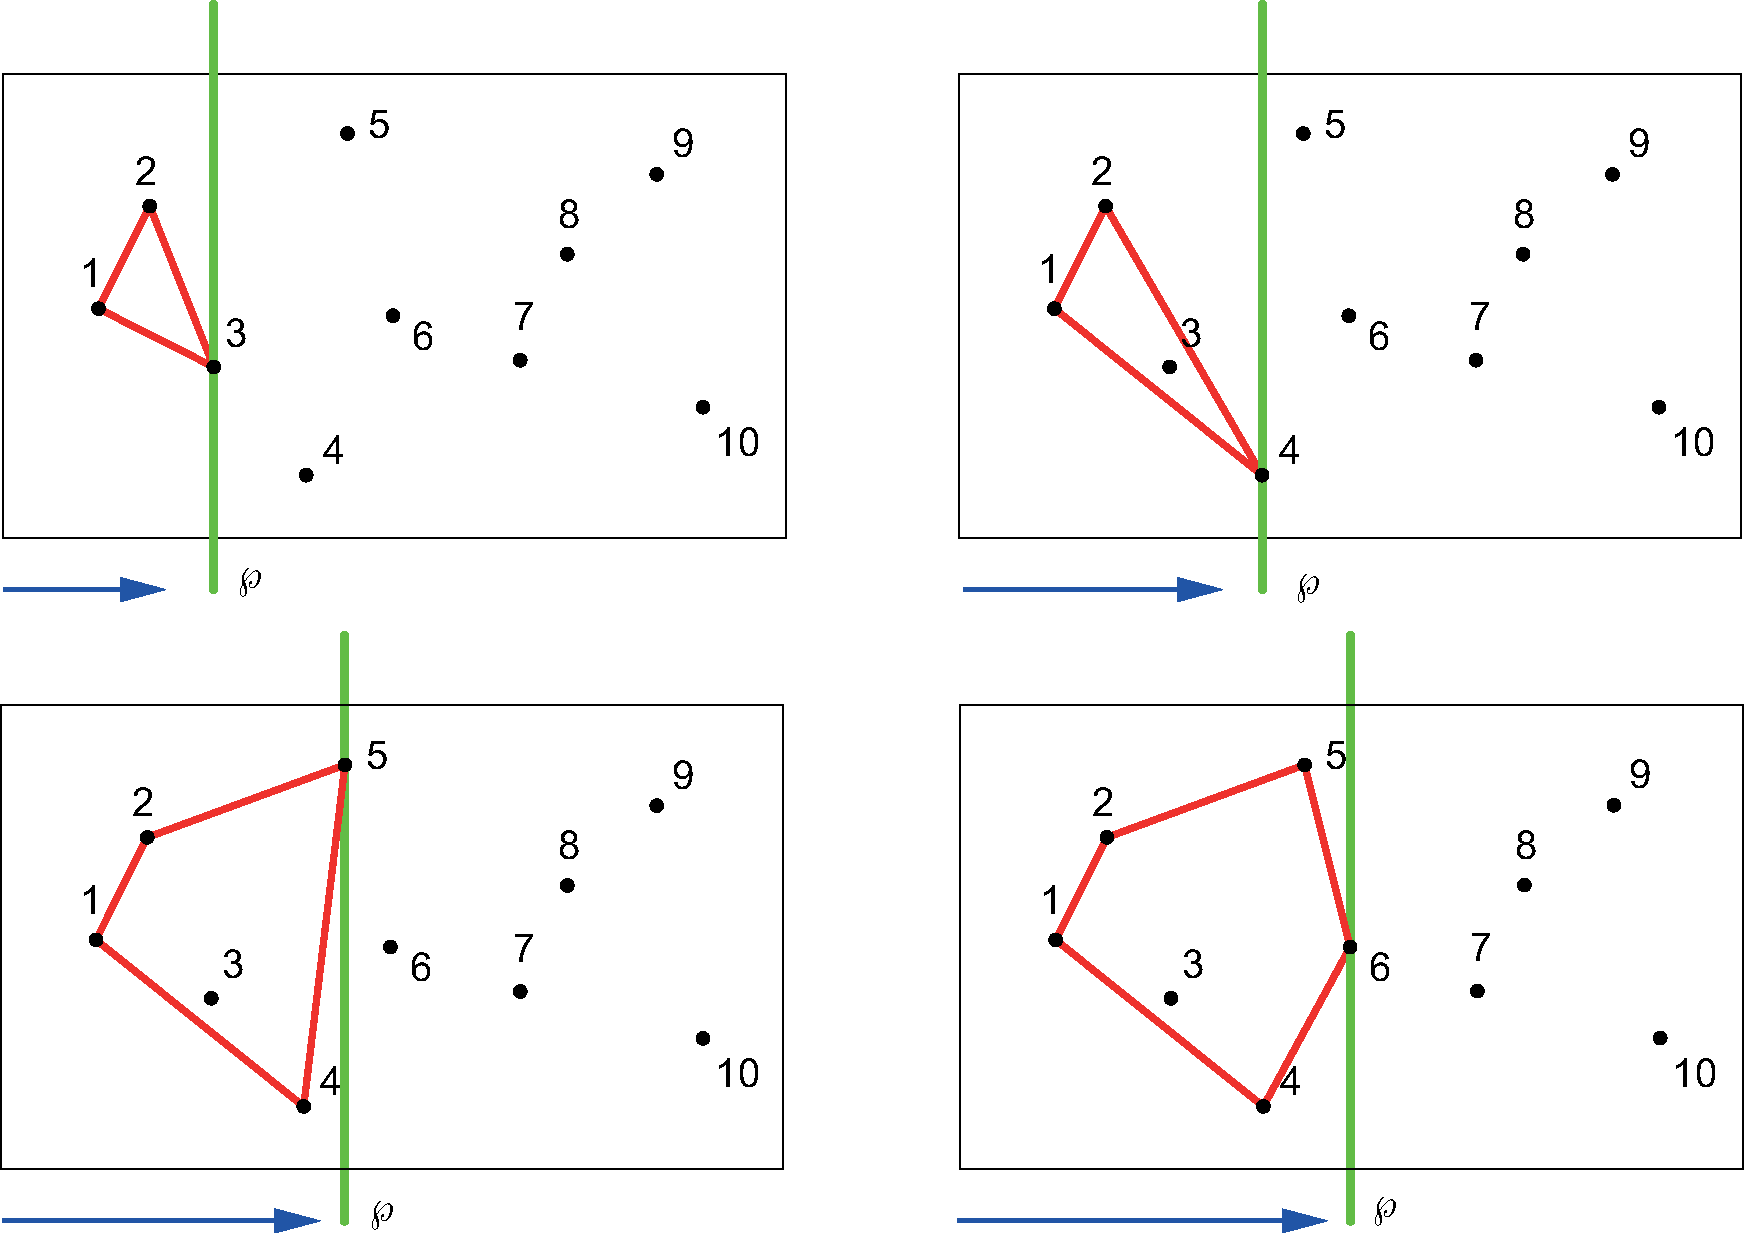
\includegraphics[scale=0.38]{E:/Tomas/LaTeX/sweep2}
\par\end{center}

\end{frame}

\begin{frame}{30. Prioritní fronta v Pythonu}

{\footnotesize Python používá implementaci prioritní fronty na bázi
haldy.}{\footnotesize\par}

{\footnotesize\medskip{}
}{\footnotesize\par}

{\footnotesize Vytvoření prioritní fronty:}{\footnotesize\par}
\begin{lyxcode}
{\footnotesize import~queue}{\footnotesize\par}

{\footnotesize Q~=~queue.PriorityQueue()~\#Volba~typu~fronty,~prioritni}{\footnotesize\par}
\end{lyxcode}
{\footnotesize\textbf{Přidání prvku do prioritní fronty:}}{\footnotesize\par}

{\footnotesize Použití metody }{\footnotesize\texttt{put()}}{\footnotesize ,
přidání na konec fronty.}{\footnotesize\par}
\begin{lyxcode}
{\footnotesize Q.put((2,~``Tuesday''))}{\footnotesize\par}

{\footnotesize Q.put((1,~``Monday''))}{\footnotesize\par}

{\footnotesize Q.put((3,~``Wednesday''))}{\footnotesize\par}
\end{lyxcode}
{\footnotesize\textbf{Odstranění prvku z priorotní fronty:}}{\footnotesize\par}

{\footnotesize Použití metody }{\footnotesize\texttt{get()}}{\footnotesize ,
odebíráme z počátku fronty.}{\footnotesize\par}
\begin{lyxcode}
{\footnotesize Q.get()}{\footnotesize\par}

{\footnotesize >\textcompwordmark >\textcompwordmark >~(1,~'Monday')}{\footnotesize\par}
\end{lyxcode}
{\footnotesize\textbf{Další metody:}}{\footnotesize\par}

{\footnotesize Počet prvků ve frontě: metoda }{\footnotesize\texttt{qsize()}}{\footnotesize .}{\footnotesize\par}

{\footnotesize Test, zda je prázdná: metoda }{\footnotesize\texttt{empty()}}{\footnotesize .}{\footnotesize\par}
\end{frame}


\subsection{N-tice}
\begin{frame}{31. N-tice (Tuple)}
 

{\scriptsize Obdoba seznamu včetně podporovaných operací.}{\scriptsize\par}

{\scriptsize Jednotlivé prvky n-tic na rozdíl od seznamů }{\scriptsize\emph{nelze
modifikovat}}{\scriptsize{} (immutable).}{\scriptsize\par}

{\scriptsize Prvky ``konstantní'', chráněny proti zápisu.}{\scriptsize\par}

{\scriptsize Výhodou vyšší rychlost.}{\scriptsize\par}

{\scriptsize Často používány jako návratové parametry funkcí.}{\scriptsize\par}

{\scriptsize{\ttfamily{}%
\begingroup
\catcode`\-=12
\begin{tabular}{|c|c|c|c|c|c|c|c|c|}
\hline 
{\scriptsize\texttt{L{[}-7{]}}} & {\scriptsize\texttt{L{[}-6{]}}} & {\scriptsize\texttt{L{[}-5{]}}} & {\scriptsize\texttt{L{[}-4{]}}} & {\scriptsize\texttt{L{[}-3{]}}} & {\scriptsize\texttt{L{[}-2{]}}} & \multicolumn{3}{c|}{{\scriptsize\texttt{L{[}-1{]}}}}\tabularnewline
\hline 
{\scriptsize\texttt{123}} & {\scriptsize\texttt{456.3}} & {\scriptsize\texttt{''Hello''}} & {\scriptsize\texttt{-37.3}} & {\scriptsize\texttt{''World''}} & {\scriptsize\texttt{False}} & {\scriptsize\texttt{-1}} & {\scriptsize\texttt{''PC''}} & {\scriptsize\texttt{False}}\tabularnewline
\hline 
{\scriptsize\texttt{L{[}0{]}}} & {\scriptsize\texttt{L{[}1{]}}} & {\scriptsize\texttt{L{[}2{]}}} & {\scriptsize\texttt{L{[}3{]}}} & {\scriptsize\texttt{L{[}4{]}}} & {\scriptsize\texttt{L{[}5{]}}} & \multicolumn{3}{c|}{{\scriptsize\texttt{L{[}6{]}}}}\tabularnewline
\hline 
\end{tabular}
\endgroup
}}{\scriptsize\par}

{\scriptsize Položky n-tice uzavřeny v kulatých závorkách.}{\scriptsize\par}
\begin{lyxcode}
{\scriptsize L~=~(123,~456.3,~-37.3)}{\footnotesize ~\#N-tice~se~3~polozkami}{\footnotesize\par}
\end{lyxcode}
{\scriptsize N-tice mohou být i vnořené.}{\scriptsize\par}
\begin{lyxcode}
{\scriptsize L~=~(123,~456.3,~''Hello'',~-37.3,~''World'',~False,~(-1,~``PC'',~False))}{\scriptsize\par}

{\scriptsize L{[}0{]}~==~L{[}-7{]}~=~123}{\scriptsize\par}

{\scriptsize L{[}2{]}{[}1{]}~==~L{[}-5{]}{[}-4{]}~=~``e''}{\scriptsize\par}

{\scriptsize K~=~L{[}2:4{]}~~~~\#Rez}{\scriptsize\par}

{\scriptsize n~=~len~L~~~~~\#Pocet~prvku}{\scriptsize\par}
\end{lyxcode}
{\scriptsize Nemají k dispozici žádné modifikační metody:}{\scriptsize\par}
\begin{lyxcode}
{\scriptsize append(),~insert(),~pop(),~del().}{\scriptsize\par}
\end{lyxcode}
\end{frame}


\subsection{Set}
\begin{frame}[plain]{32. Množina (Set)}
 

{\footnotesize Neuspořádaná množina unikátních objektů (nemohou být
duplicitní).}{\footnotesize\par}

{\footnotesize Unikátnost zajištěna hashovací funkcí $h$}{\footnotesize\par}

{\footnotesize
\[
(a_{i},x_{i}),\qquad a_{i}=h(x_{i}).
\]
}{\footnotesize\par}

{\footnotesize K prvkům nelze přistupovat přímo (index), nelze provádět
řezy.}{\footnotesize\par}

{\footnotesize Prvky množiny lze modifikovat.}{\footnotesize\par}
\begin{center}
{\footnotesize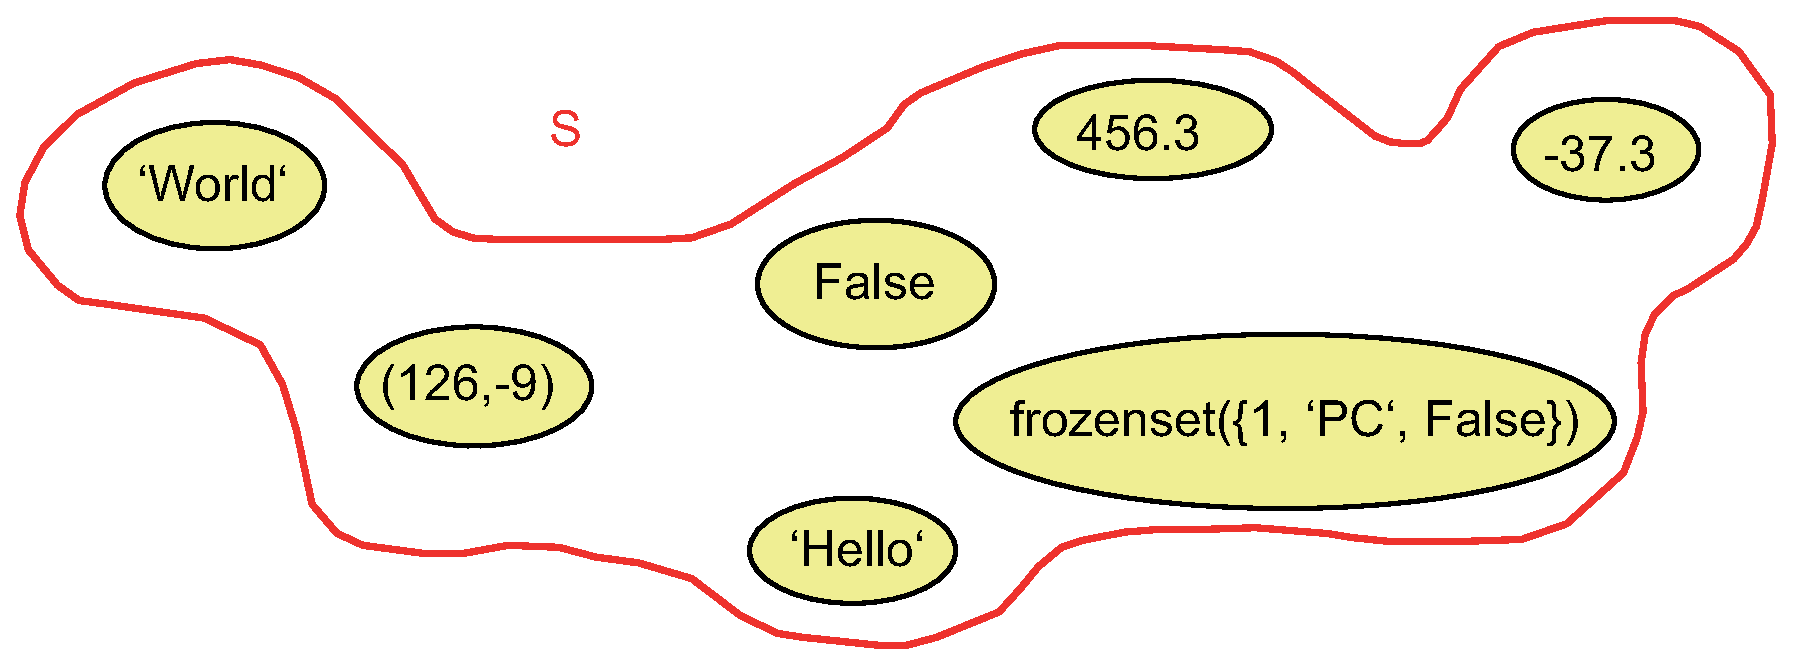
\includegraphics[scale=0.25]{set}}{\footnotesize\par}
\par\end{center}

{\footnotesize Položky množiny uzavřeny v lomených závorkách.}{\footnotesize\par}

{\footnotesize Množiny mohou být vnořené: tvořeny n-ticemi, podmnožinami
(frozensets).}{\footnotesize\par}
\begin{lyxcode}
{\footnotesize S~=~\{(-126,9),~456.3,~''Hello'',~-37.3,~''World'',~False,~}{\footnotesize\par}

{\footnotesize ~~~~~frozenset(-1,~``PC'',~False)\}~~\#Vnorena~mnozina}{\footnotesize\par}

{\footnotesize L~=~(1,2,3)}{\footnotesize\par}

{\footnotesize S~=~set(L)~~\#Mnozina~z~entice}{\footnotesize\par}
\end{lyxcode}
\end{frame}

\begin{frame}{33. Vlastnosti množin}
 

V Pythonu implementovány s využitím Hash Table.

Složitost operací $O(N)$.

Ve většině případů výkonnější než seznam.\medskip{}

+ Přidávání prvku do množiny $\varTheta(1)$.

+ Hledání prvku v množině $\varTheta(1)$.

+ Mazání prvku $\varTheta(1)$.\bigskip{}

- V nepříznivých případech kolize: operace nemají konstantní složitost.

- Nastává pro ``nevhodná'' data. \bigskip{}

\textbf{Použití množin:}

Použití pro práci s velkými daty.

V průměrném případě mnohem efektivnější než jiné datové struktury
(hledání).

Umožňují booleovské operace s prvky.
\end{frame}

\begin{frame}{34. Základní operace s množinami}

{\scriptsize Vytvoření prázdné množiny:}{\scriptsize\par}
\begin{lyxcode}
{\scriptsize S~=~\{\}~~~~S~=~set()}{\scriptsize\par}
\end{lyxcode}
{\scriptsize Délka seznamu: příkaz }{\scriptsize\texttt{len()}}{\scriptsize\par}
\begin{lyxcode}
{\scriptsize n~=~len(S)}{\scriptsize\par}
\end{lyxcode}
{\scriptsize Přidání prvku: metoda }{\scriptsize\texttt{add()}}{\scriptsize\par}
\begin{lyxcode}
{\scriptsize S.add(-126.9)}{\scriptsize\par}
\end{lyxcode}
{\scriptsize Přidání jiné podmnožiny: metoda }{\scriptsize\texttt{insert()}}{\scriptsize\par}
\begin{lyxcode}
{\scriptsize S.insert(\{456.3,-137.3,''Hello''\})}{\scriptsize\par}
\end{lyxcode}
{\scriptsize Nalezení položky na pozici v množině: funkce }{\scriptsize\texttt{in}}{\scriptsize\par}
\begin{lyxcode}
{\scriptsize r~=~-137~in~S~\#True~nebo~False}{\scriptsize\par}
\end{lyxcode}
{\scriptsize Odstranění posledního prvku z množiny: metoda }{\scriptsize\texttt{pop()}}{\scriptsize\par}
\begin{lyxcode}
{\scriptsize n~=~S.pop()}{\scriptsize\par}
\end{lyxcode}
{\scriptsize Odstranění položky $p$ z množiny: metody }{\scriptsize\texttt{remove(),
discard()}}{\scriptsize\par}
\begin{lyxcode}
{\scriptsize S.remove(-137)~~\#Pokud~S~neobsahuje~p,~vyjimka}{\scriptsize\par}

{\scriptsize S.discard(-137)~\#Vyjimka~neprobehne}{\scriptsize\par}
\end{lyxcode}
\end{frame}

\begin{frame}{35. Množinové operace v Pythonu}

{\scriptsize 4 základní operace booleovské operace s množinami:}{\scriptsize\par}
\begin{itemize}
\item {\scriptsize Union: $C=A\cup B$.}{\scriptsize\par}
\item {\scriptsize Intersection: $C=A\cap B$.}{\scriptsize\par}
\item {\scriptsize Difference: $C=A\cap\overline{B}$, $B\cap\overline{A}$.}{\scriptsize\par}
\item {\scriptsize Symmetric Difference: $C=\left(A\cup B\right)\cap\left(\overline{A\cap B}\right)$.}{\scriptsize\par}
\end{itemize}
{\scriptsize Konjunkce $\cap$, disjunkce $\cup$, negace $\overline{\cdot}$
resp $!$.}{\scriptsize\par}
\begin{center}
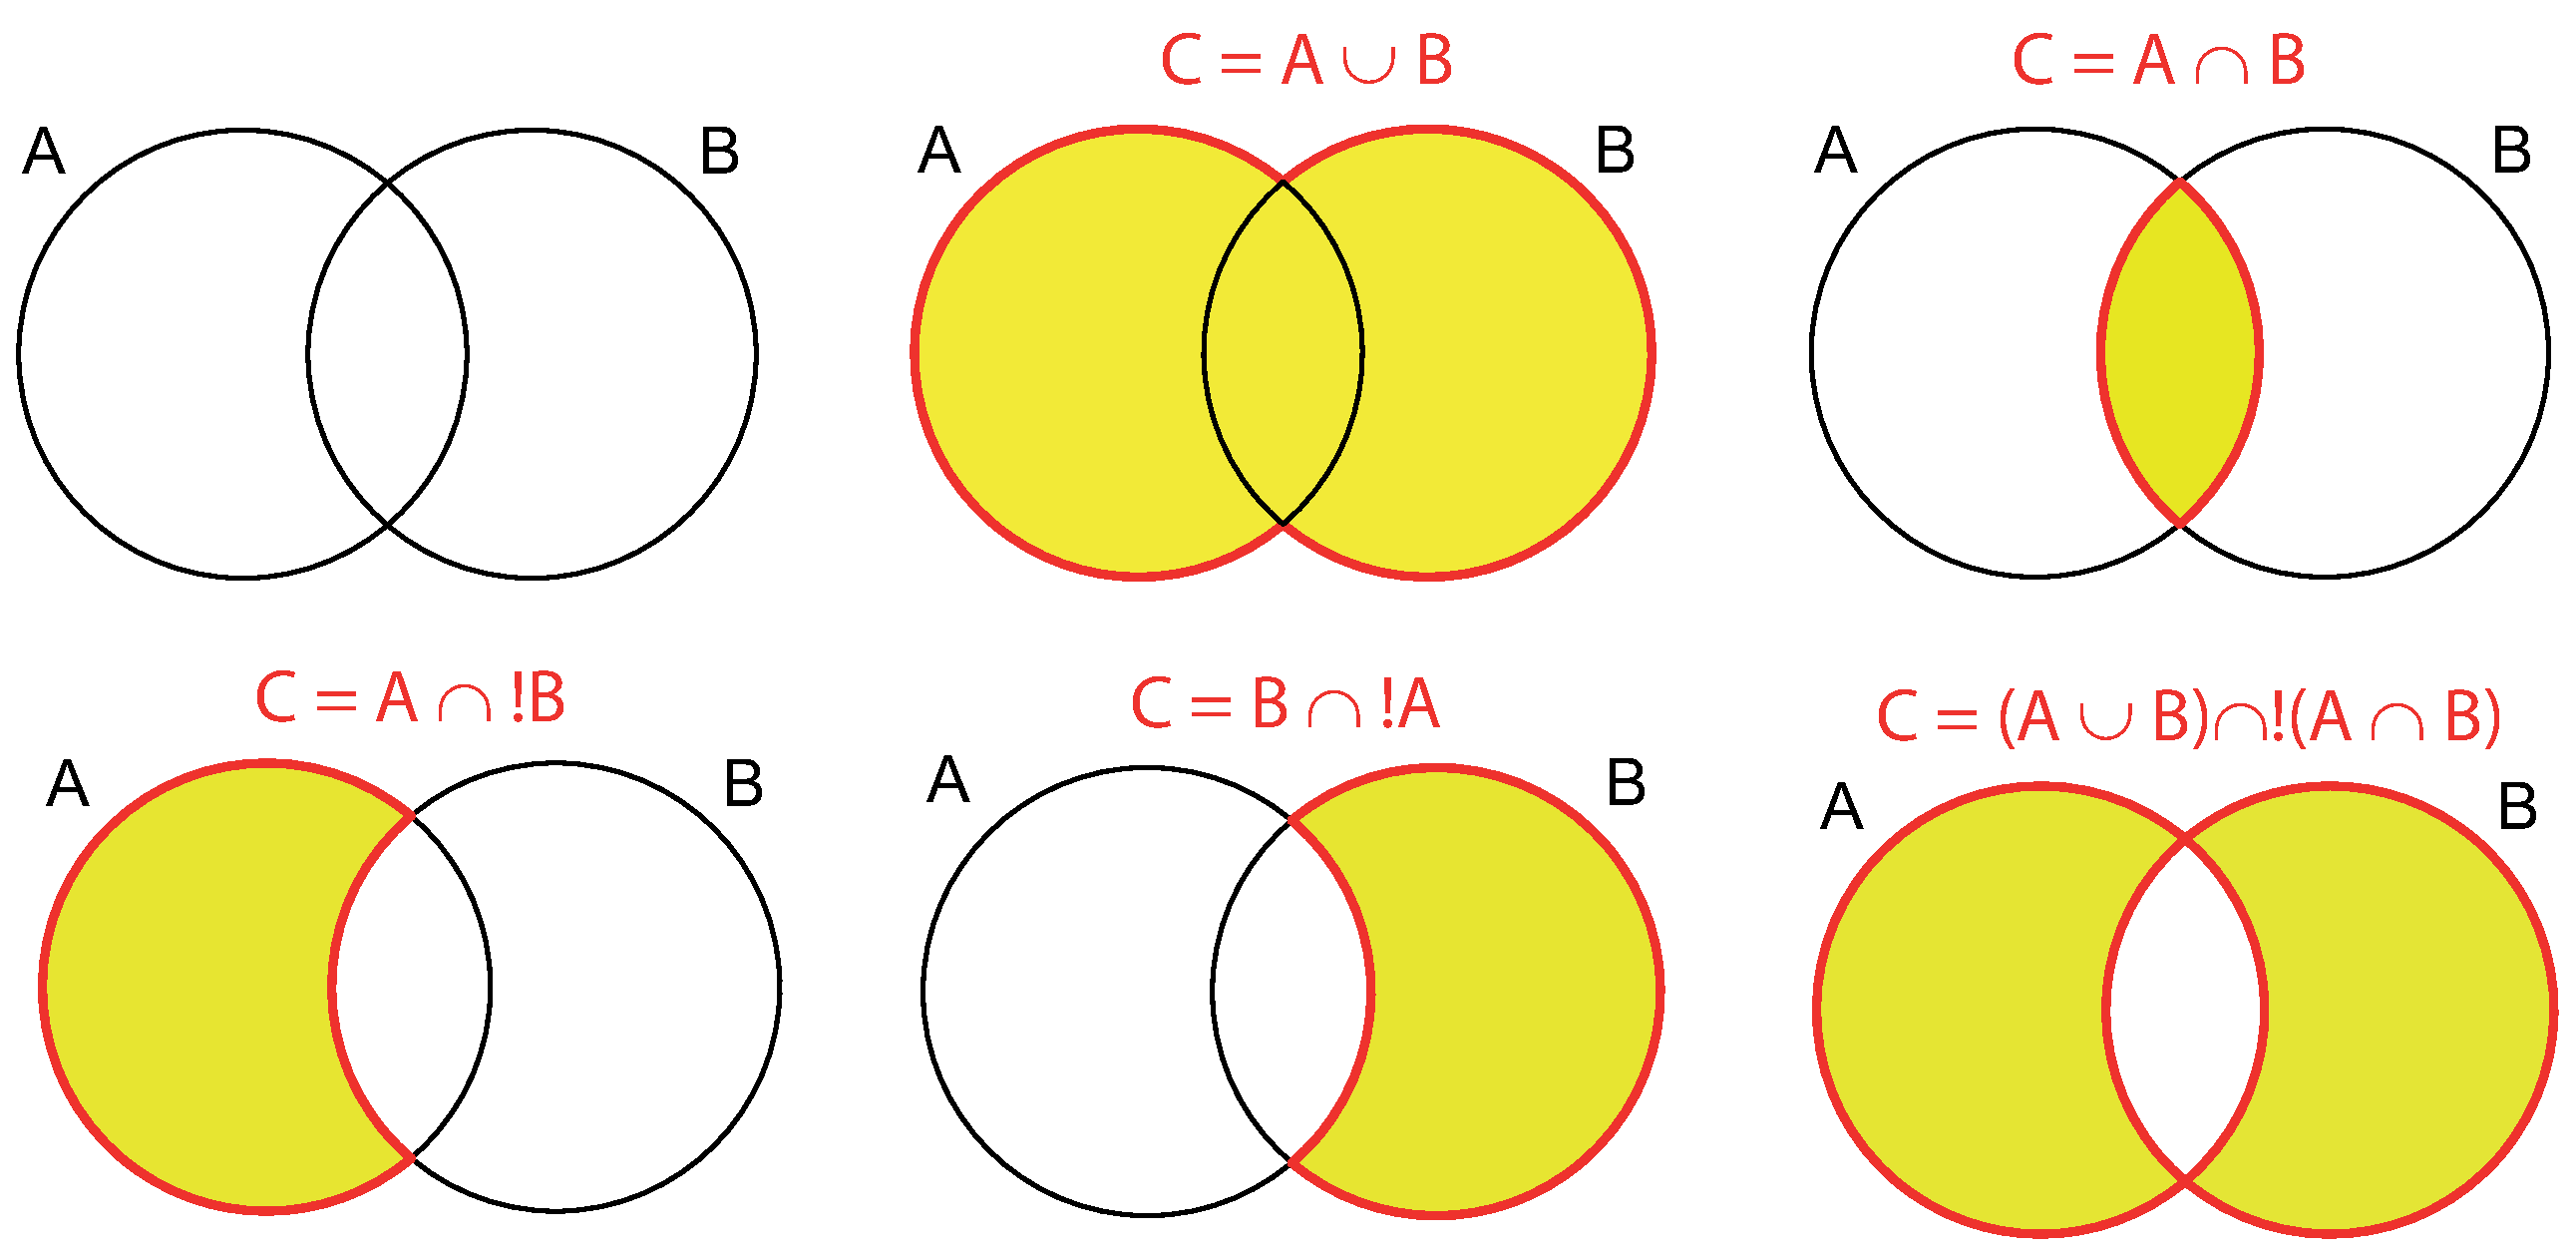
\includegraphics[scale=0.25]{set_operations}
\par\end{center}

\end{frame}

\begin{frame}{36. Sjednocení (Union)}

Komutativita (symetrie):
\[
A\cup B=B\cup A.
\]

Asociativita

\[
A\cup\left(B\cup C\right)=\left(A\cup B\right)\cup C.
\]

Příklad: 
\begin{lyxcode}
A~=~\{\textquotedbl H\textquotedbl ,~\textquotedbl e\textquotedbl ,~\textquotedbl l\textquotedbl ,~\textquotedbl l\textquotedbl ,~\textquotedbl o\textquotedbl\}

B~=~\{\textquotedbl w\textquotedbl ,~\textquotedbl o\textquotedbl ,~\textquotedbl r\textquotedbl ,~\textquotedbl l\textquotedbl ,~\textquotedbl d\textquotedbl\}

C~=~A.union(B))

>\textcompwordmark >\textcompwordmark >~\{'d',~'o',~'H',~'e',~'w',~'r',~'l'\}~~
\end{lyxcode}
\end{frame}

\begin{frame}{37. Průnik (Intersection)}

Komutativita (symetrie):
\[
A\cap B=B\cap A.
\]

Asociativita

\[
A\cap\left(B\cap C\right)=\left(A\cap B\right)\cap C.
\]

Příklad: 
\begin{lyxcode}
A~=~\{\textquotedbl H\textquotedbl ,~\textquotedbl e\textquotedbl ,~\textquotedbl l\textquotedbl ,~\textquotedbl l\textquotedbl ,~\textquotedbl o\textquotedbl\}

B~=~\{\textquotedbl w\textquotedbl ,~\textquotedbl o\textquotedbl ,~\textquotedbl r\textquotedbl ,~\textquotedbl l\textquotedbl ,~\textquotedbl d\textquotedbl\}

C~=~A.intersection(B))

>\textcompwordmark >\textcompwordmark >~\{'o',~'l'\}~~
\end{lyxcode}
\end{frame}

\begin{frame}[plain]{38. Rozdíl (Difference)}

{\small Neplatí komutativita
\begin{align*}
A\ominus B & \neq B\ominus A,\qquad A\cap\overline{B}\neq B\cap\overline{A},
\end{align*}
}{\small\par}

{\small ani asociativita}{\small\par}

{\small
\begin{align*}
A\ominus(B\ominus C) & \neq(A\ominus B)\ominus C,\qquad A\cap(\overline{B\cap\overline{C})}\neq(A\cap\overline{B})\cap\overline{C}.
\end{align*}
Avšak
\begin{align*}
A\ominus(B\cap C) & =(A\ominus B)\cup(A\ominus C),\qquad A\cap(\overline{B\cap C})=(A\cap\overline{B})\cup(A\cap\overline{C}),\\
A\ominus(B\cup C) & =(A\ominus B)\cap(A\ominus C),\qquad A\cap(\overline{B\cup C})=(A\cap\overline{B})\cap(A\cap\overline{C}),
\end{align*}
}{\small\par}

{\small Příklad: }{\small\par}
\begin{lyxcode}
{\small A~=~\{\textquotedbl H\textquotedbl ,~\textquotedbl e\textquotedbl ,~\textquotedbl l\textquotedbl ,~\textquotedbl l\textquotedbl ,~\textquotedbl o\textquotedbl\}}{\small\par}

{\small B~=~\{\textquotedbl w\textquotedbl ,~\textquotedbl o\textquotedbl ,~\textquotedbl r\textquotedbl ,~\textquotedbl l\textquotedbl ,~\textquotedbl d\textquotedbl\}}{\small\par}

{\small C~=~A.difference(B))}{\small\par}

{\small D~=~B.difference(A))}{\small\par}

{\small >\textcompwordmark >\textcompwordmark >~\{'e',~'H'\}~~~~~~~~~~~~~~~~~~~~~~~~~~~~~~~~~~~~~~~~~~~~~~~~~~~~~~~~~~~~~~~~~~~~~~~~~~~~~~~~~~~~~~~~~~~~~~~~~~~~~~~~~~~}{\small\par}

{\small >\textcompwordmark >\textcompwordmark >~\{'w',~'d',~'r'\}~~}{\small\par}
\end{lyxcode}
\end{frame}

\begin{frame}{39. Symmetric Difference (XOR)}

{\footnotesize Geometrická představa: sjednocení - průnik.}{\footnotesize\par}

{\footnotesize Komutativita (symetrie):
\[
A\bigtriangleup B=B\bigtriangleup A\qquad\left(A\cup B\right)\cap\left(\overline{A\cap B}\right)=\left(B\cup A\right)\cap\left(\overline{B\cap A}\right).
\]
}{\footnotesize\par}

{\footnotesize Asociativita}{\footnotesize\par}

{\footnotesize
\begin{align*}
A\bigtriangleup\left(B\bigtriangleup C\right) & =\left(A\bigtriangleup B\right)\bigtriangleup C,
\end{align*}
kde
\begin{align*}
A\bigtriangleup\left(B\bigtriangleup C\right) & =(A\cup[\left(B\cup C\right)\cap\overline{(B\cap C)}])\cap(\overline{A\cap[\left(B\cup C\right)\cap\overline{(B\cap C)}]},\\
\left(A\bigtriangleup B\right)\bigtriangleup C & =([\left(A\cup B\right)\cap(\overline{A\cap B})]\cup C)\cap(\overline{[\left(A\cup B\right)\cap(\overline{A\cap B})]\cap C}).
\end{align*}
}{\footnotesize\par}

{\footnotesize Příklad: }{\footnotesize\par}
\begin{lyxcode}
{\footnotesize A~=~\{\textquotedbl H\textquotedbl ,~\textquotedbl e\textquotedbl ,~\textquotedbl l\textquotedbl ,~\textquotedbl l\textquotedbl ,~\textquotedbl o\textquotedbl\}}{\footnotesize\par}

{\footnotesize B~=~\{\textquotedbl w\textquotedbl ,~\textquotedbl o\textquotedbl ,~\textquotedbl r\textquotedbl ,~\textquotedbl l\textquotedbl ,~\textquotedbl d\textquotedbl\}}{\footnotesize\par}

{\footnotesize C~=~A.symmetric\_difference(B))}{\footnotesize\par}

{\footnotesize >\textcompwordmark >\textcompwordmark >~\{'r',~'w',~'d',~'e',~'H'\}~~~}{\footnotesize\par}
\end{lyxcode}
\end{frame}


\subsection{Slovník}
\begin{frame}{40. Slovník (Dictionary)}

{\footnotesize Neuspořádaná množina unikátních dvojic}{\footnotesize\par}
\begin{lyxcode}
{\footnotesize (klíč~:~hodnota)}{\footnotesize\par}
\end{lyxcode}
{\footnotesize Jako klíč lze použít pouze }{\footnotesize\emph{immutable
objekty}}{\footnotesize .}{\footnotesize\par}

{\footnotesize Klíč unikátní v celém seznamu.}{\footnotesize\par}

{\footnotesize Hodnota může být reprezentována libovolným typem.}{\footnotesize\par}

{\footnotesize U dvojice (záznamu) lze měnit pouze hodnotu.}{\footnotesize\par}

{\footnotesize\bigskip{}
}{\footnotesize\par}

{\footnotesize Implementován s využitím }{\footnotesize\emph{hashovací
tabulky,}}{\footnotesize{} operace }v $\varTheta(1)$.
\begin{center}
{\footnotesize\includegraphics[scale=0.25]{dictionary}}{\footnotesize\par}
\par\end{center}

{\footnotesize Použití: rychlé vyhledání hodnoty dle klíče.}{\footnotesize\par}

{\footnotesize V jiných programovacích jazycích známa jako map (unordered
set).}{\footnotesize\par}
\end{frame}

\begin{frame}[plain]{41. Operace se slovníkem}

{\tiny Vytvoření slovníku:}{\tiny\par}
\begin{lyxcode}
{\tiny D~=~\{1~:~\textquotedbl World\textquotedbl ,~-7~:~False,~3~:~\textquotedbl Wednesday\textquotedbl ,~19~:~-37.3,~'A'~:~{[}-126,~9{]},}{\tiny\par}

{\tiny ~~~~'My'~:~456.3,~'False'~:~Hello,~'World'~:~{[}1,~'PC',~False{]}\}}{\tiny\par}
\end{lyxcode}
{\tiny Délka slovníku: funkce }{\tiny\texttt{len()}}{\tiny\par}
\begin{lyxcode}
{\tiny n~=~len(D)}{\tiny\par}
\end{lyxcode}
{\tiny Přidání prvku: metoda }{\tiny\texttt{add()}}{\tiny\par}
\begin{lyxcode}
{\tiny D{[}13{]}~=~'New~value'}{\tiny\par}
\end{lyxcode}
{\tiny Nalezení položky ve slovníku: funkce }{\tiny\texttt{in}}{\tiny\par}
\begin{lyxcode}
{\tiny r~=~-137~in~S~\#True~nebo~False}{\tiny\par}
\end{lyxcode}
{\tiny Nalezení hodnoty dle klíče: metoda }{\tiny\texttt{get()}}{\tiny\par}
\begin{lyxcode}
{\tiny r~=~D.get(13)}{\tiny\par}
\end{lyxcode}
{\tiny Odstranění položky ze slovníku: funkce }{\tiny\texttt{del()}}{\tiny\par}
\begin{lyxcode}
{\tiny del(D,~-137)}{\tiny\par}
\end{lyxcode}
{\tiny Procházení slovníku:}{\tiny\par}
\begin{lyxcode}
{\tiny for~d~in~D~~~~~~~~~~\#Prochazeni~po~klicich}{\tiny\par}

{\tiny for~d~in~D.values()~\#Prochazeni~po~hodnotach}{\tiny\par}

{\tiny for~d~in~D.items()~~\#Prochazeni~po~klicich~i~hodnotach}{\tiny\par}
\end{lyxcode}
{\tiny Slovník podporuje všechny }{\tiny\emph{množinové operace}}{\tiny .}{\tiny\par}
\end{frame}

\begin{frame}[plain]{42. Dynamické datové struktury a typová kontrola}

{\scriptsize Podpora Type Hints i pro dynanamické datové struktury.}{\scriptsize\par}

{\scriptsize Tyto informace lze použít pro typovou kontrolu.}{\scriptsize\par}
\begin{lyxcode}
{\scriptsize from~typing~import~List,~Tuple,~Dict~~~~~~~~~~~~~~~~~}{\scriptsize\par}

{\scriptsize l:~List{[}str{]}~=~{[}'a',~'b',~'c'{]}~~~~~~~~~~~~~~~~\#Seznam~objektu~typu~string}{\scriptsize\par}

{\scriptsize t:~Tuple{[}int,~int,~int{]}~=~(1,~2,~3)~~~~~~~~~~~\#N-tice~objektu~typu~int}{\scriptsize\par}

{\scriptsize d:~Dict{[}str,~int{]}~=~\{'a':~1,~'b':~2,~'c'~:3\}~~\#Slovnik,~key=string,~val~=~~int}{\scriptsize\par}
\end{lyxcode}
{\scriptsize Typová kontrola, odhalení chyby:}{\scriptsize\par}
\begin{lyxcode}
{\scriptsize l{[}0{]}~=~7~~~~~~~~~~~~~\#Prirazeni~objektu~typu~int,~ocekavano~str~\medskip{}
}{\scriptsize\par}
\end{lyxcode}
\begin{center}
\includegraphics[scale=0.18]{stat_kontrola2}
\par\end{center}

\end{frame}


\end{document}
